\chapter{Mécanisme de pyrolyse simplifié}
\label{an:simplification-norinaga}

\begin{figure}[!h]
  \centering\resizebox{0.75\textwidth}{!}{%
    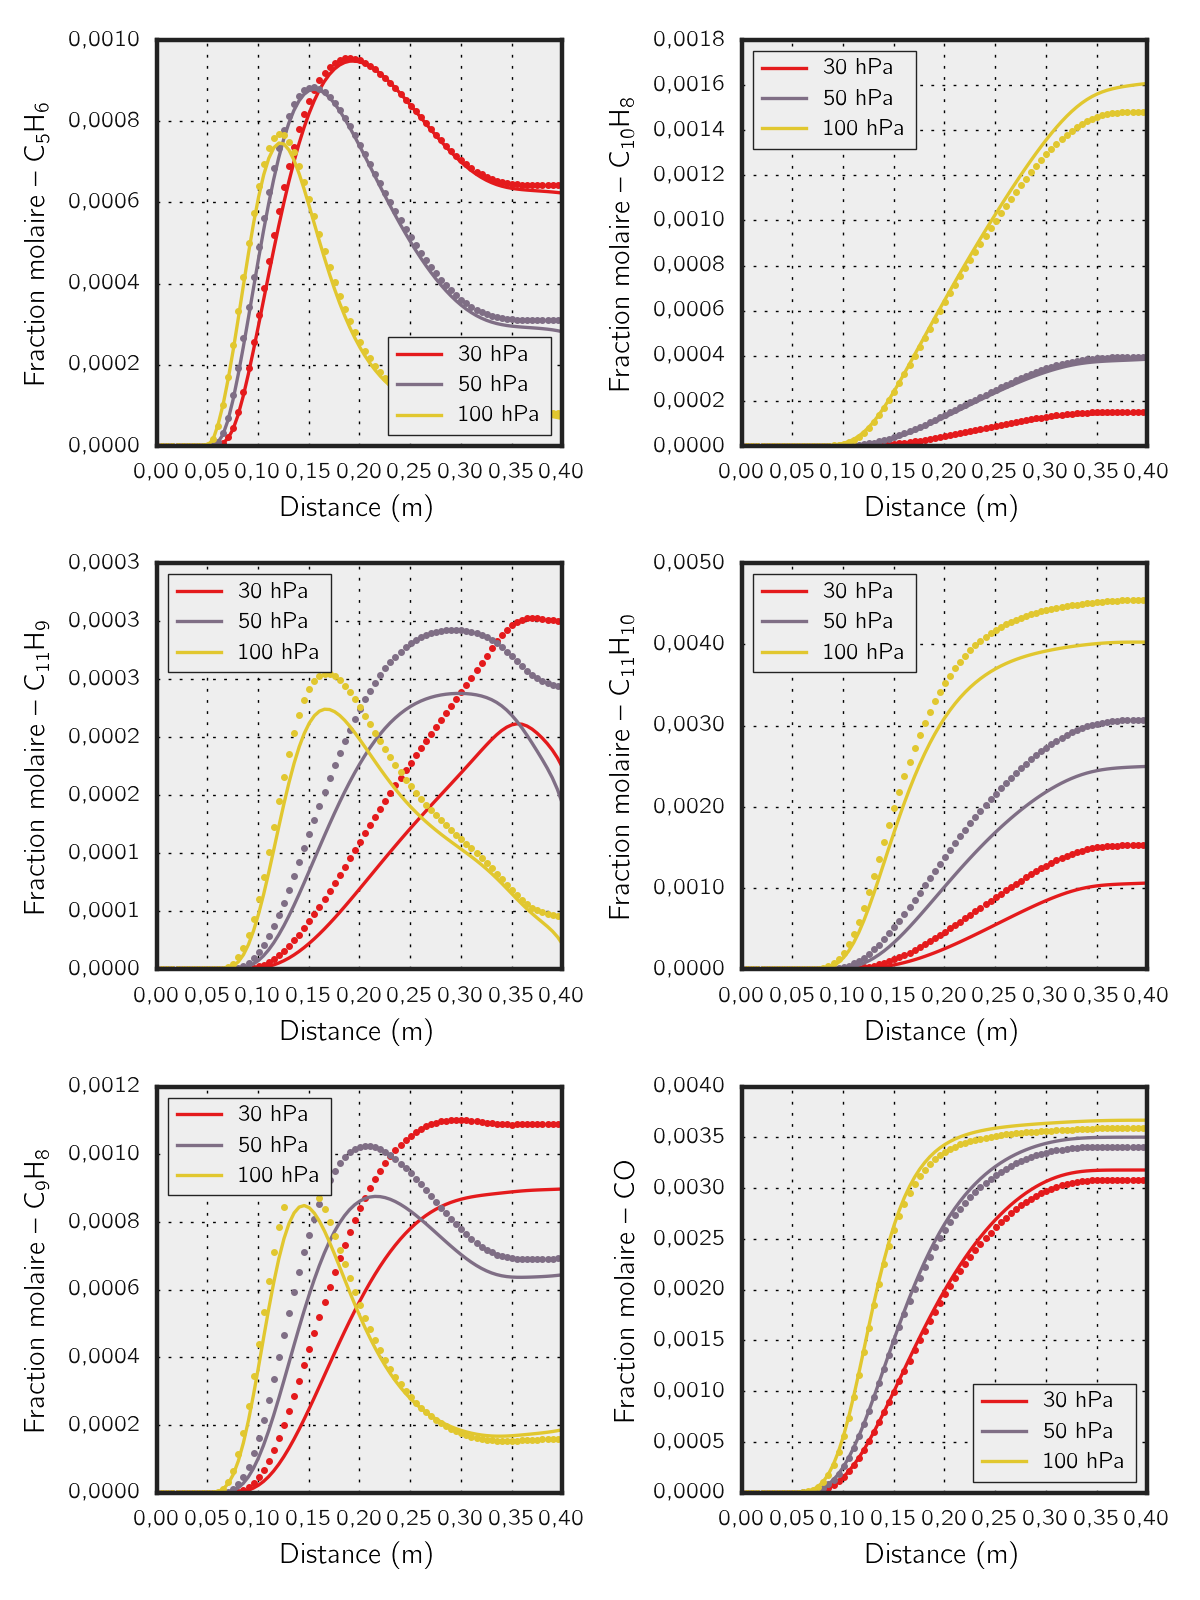
\includegraphics{figures/ann-kinetics-norinaga-simplification-1173K-hap}}

  \caption{\label{norinaga-comparison-simplification-1173K-hap}Comparaison entre les intégrations du mécanisme simplifié (points) et le mécanisme de \citet{Norinaga2009} (traits) de pyrolyse de l'acétylène dans un réacteur de type piston avec un palier de température à \SI{1173}{\kelvin}. Cette figure vise à montrer l'accord au moins qualitatif pour quelques espèces lourdes retenues dans le mécanisme simplifié ainsi que pour le \ch{CO}. On doit remarquer le très bon accord quantitatif obtenu pour le naphtalène \ch{C10H8}, un des principaux responsables de la formation des hydrocarbures polycycliques.}
\end{figure}

\begin{figure}[h]
  \centering\resizebox{0.75\textwidth}{!}{%
    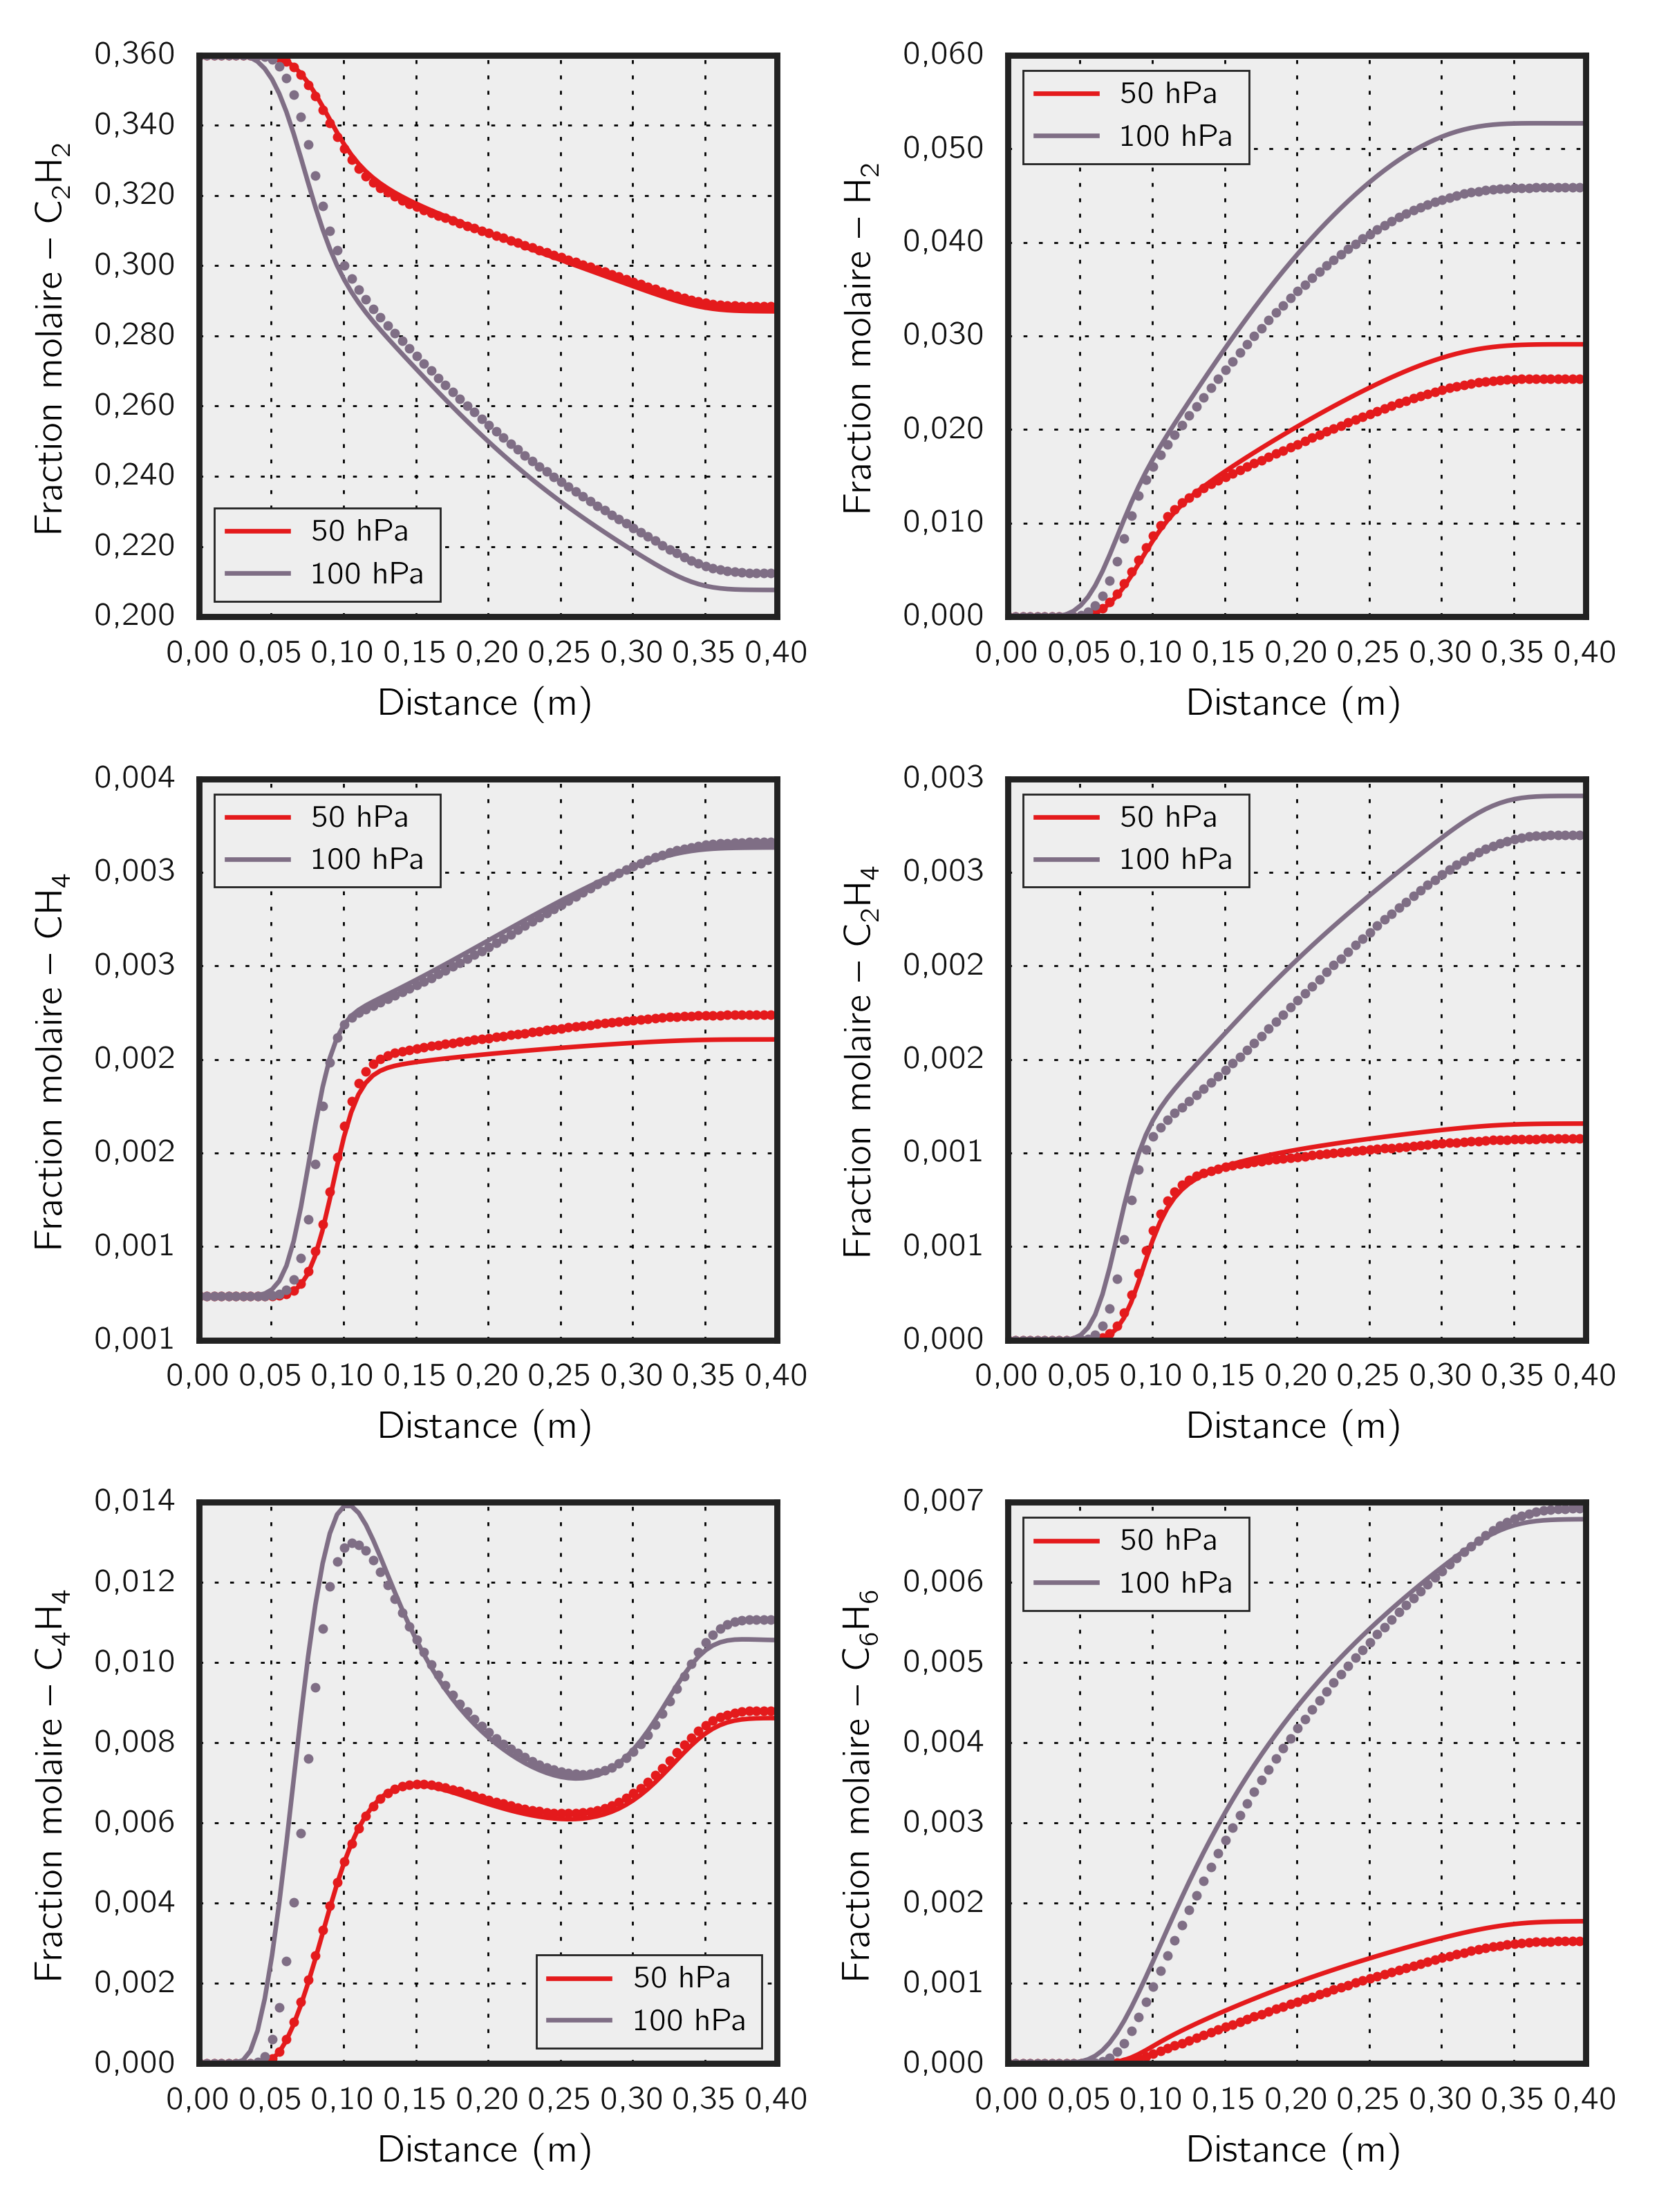
\includegraphics{figures/ann-kinetics-norinaga-simplification-1273K}}

  \caption{\label{norinaga-comparison-simplification-1273K}Comparaison entre les intégrations du mécanisme simplifié (points) et le mécanisme de \citet{Norinaga2009} (traits) de pyrolyse de l'acétylène dans un réacteur de type piston avec un palier de température à \SI{1273}{\kelvin}. Cependant le mécanisme simplifié a été obtenu avec des simulations réalisées à \SI{1173}{\kelvin}. Une bonne correspondance est trouvée.}
\end{figure}

\clearpage

\begin{verbatim}
! Mécanisme cinétique simplifié.
! Nombre d'espèces 40 + N2
! Nombre de réactions 161
!
! Mécanisme source: 
!     Norinaga et al., J. Anal. Appl. Pyrolysis 86 (2009) 148–160
!
! Données cinétiques:
!     k = A * T**b * exp (-Ea/RT)        A          b       Ea
!                                    (cm,mol,s)    -     kJ/mol
! 
! Pour les données thermodynamiques, veuillez consulter le mécanisme source.
!

ELEMENTS
C H O N
END

SPECIES
C2H2      H2        H         CH4       CH3       C2H4      C2H3      C2H6
C2H5      C4H2      C4H4      C6H6      C6H5      C3H6      C3H3      AC3H5
AC3H4     PC3H4     SC3H5     C4H6      C4H61     C4H612    I-C4H51   I-C4H3
C5H6      C5H5      C7H7      C8H8      C9H8      C9H7      A1C2H     A1C2H3
A2        CO        A2CH3-2   A2CH2-2   CH3COCH3  CH3COCH2  CH2CO     CH3CO
N2
END

REACTIONS KJOULES/MOLE
! H ****************************************************************************
H + H + M <=> H2 + M                     1.000000e+18     -1.000    0.000000e+00
  C2H6 / 3.00 / CH4 / 2.00 / H2 / 0.00 / 
H + H + H2 <=> 2 H2                      9.200000e+16     -0.600    0.000000e+00
! C1 ***************************************************************************
CH3 + H (+M) <=> CH4 (+M)                1.270000e+16     -0.630    1.600000e+00
  LOW  /                               2.477000e+33     -4.760    1.021000e+01 /
  TROE /    0.78300    7.400000e+01    2.941000e+03    6.964000e+03 /
  C2H6 / 3.00 / CH4 / 2.00 / H2 / 2.00 / 
CH3 + CH3 (+M) <=> C2H6 (+M)             2.120000e+16     -0.970    2.590000e+00
  LOW  /                               1.770000e+50     -9.670    2.603000e+01 /
  TROE /    0.53200    1.510000e+02    1.038000e+03    4.970000e+03 /
  C2H6 / 3.00 / CH4 / 2.00 / H2 / 2.00 / 
CH3 + CH4 <=> C2H5 + H2                  1.000000e+13      0.000    9.624000e+01
CH3 + CH4 <=> C2H6 + H                   8.000000e+13      0.000    1.673700e+02
CH3 + CH3 <=> C2H4 + H2                  1.000000e+16      0.000    1.340200e+02
CH3 + CH3 <=> C2H5 + H                   4.990000e+12      0.100    4.435000e+01
CH3 + I-C4H3 <=> C5H6                    1.000000e+12      0.000    0.000000e+00
CH3 + PC3H4 <=> C3H3 + CH4               1.000000e+12      0.000    3.347000e+01
CH3 + SC3H5 <=> AC3H4 + CH4              1.000000e+11      0.000    0.000000e+00
CH4 + H <=> CH3 + H2                     6.600000e+08      1.620    4.536000e+01
! C2 ***************************************************************************
C2H2 + H (+M) <=> C2H3 (+M)              5.600000e+12      0.000    1.004000e+01
  LOW  /                               3.800000e+40     -7.270    3.021000e+01 /
  TROE /    0.75100    9.850000e+01    1.302000e+03    4.167000e+03 /
  C2H6 / 3.00 / CH4 / 2.00 / H2 / 2.00 / 
C2H3 + H (+M) <=> C2H4 (+M)              6.080000e+12      0.270    1.170000e+00
  LOW  /                               1.400000e+30     -3.860    1.389000e+01 /
  TROE /    0.78200    2.075000e+02    2.663000e+03    6.095000e+03 /
  C2H6 / 3.00 / CH4 / 2.00 / H2 / 2.00 / 
C2H4 (+M) <=> C2H2 + H2 (+M)             8.000000e+12      0.440    3.714300e+02
  LOW  /                               7.000000e+50     -9.310    4.178300e+02 /
  TROE /    0.73500    1.800000e+02    1.035000e+03    5.417000e+03 /
  C2H6 / 3.00 / CH4 / 2.00 / H2 / 2.00 / 
C2H4 + H (+M) <=> C2H5 (+M)              1.080000e+12      0.454    7.620000e+00
  LOW  /                               1.200000e+42     -7.620    2.916000e+01 /
  TROE /    0.97500    2.100000e+02    9.870000e+02    4.374000e+03 /
  C2H6 / 3.00 / CH4 / 2.00 / H2 / 2.00 / 
C2H5 + H (+M) <=> C2H6 (+M)              5.210000e+17     -0.990    6.610000e+00
  LOW  /                               1.990000e+41     -7.080    2.797000e+01 /
  TROE /    0.84200    1.250000e+02    2.219000e+03    6.882000e+03 /
  C2H6 / 3.00 / CH4 / 2.00 / H2 / 2.00 / 
C2H2 + C2H2 <=> C4H2 + H2                1.500000e+13      0.000    1.786700e+02
C2H2 + C2H2 <=> C4H4                     5.500000e+12      0.000    1.546500e+02
C2H2 + C2H3 <=> C4H4 + H                 4.600000e+16     -1.250    3.515000e+01
C2H2 + C4H4 <=> C6H5 + H                 1.000000e+09      0.000    1.260000e+02
C2H2 + C4H4 <=> C6H6                     4.470000e+11      0.000    1.260000e+02
C2H2 + C6H5 <=> A1C2H + H                8.320000e+22     -2.680    7.281000e+01
C2H2 + C7H7 <=> C9H8 + H                 1.000000e+11      0.000    2.929000e+01
C2H2 + C9H7 <=> A2CH2-2                  5.000000e+11      0.000    4.325000e+01
C2H2 + CH3 <=> AC3H4 + H                 2.870000e+21     -2.740    1.037700e+02
C2H2 + CH3 <=> AC3H5                     1.400000e+04      2.210    6.904000e+01
C2H2 + CH3 <=> H + PC3H4                 1.000000e+13     -0.530    5.607000e+01
C2H2 + H2 <=> C2H4                       1.410000e+41     -9.060    2.139450e+02
C2H3 + C2H3 <=> C2H2 + C2H4              1.440000e+13      0.000    0.000000e+00
C2H3 + C2H3 <=> C4H6                     1.500000e+52    -11.970    6.737000e+01
C2H3 + C2H4 <=> C4H6 + H                 7.400000e+14     -0.660    3.523000e+01
C2H3 + C2H5 <=> C2H2 + C2H6              4.820000e+11      0.000    0.000000e+00
C2H3 + C2H6 <=> C2H4 + C2H5              1.500000e+13      0.000    4.180000e+01
C2H3 + C3H3 <=> C5H5 + H                 9.630000e+40     -7.800    1.205900e+02
C2H3 + C3H6 <=> AC3H5 + C2H4             2.200000e+00      3.500    1.960000e+01
C2H3 + C3H6 <=> C2H4 + SC3H5             1.300000e+00      3.500    4.560000e+01
C2H3 + C3H6 <=> C4H6 + CH3               7.230000e+11      0.000    2.096000e+01
C2H3 + C4H4 <=> C2H4 + I-C4H3            5.000000e+11      0.000    6.820000e+01
C2H3 + C5H6 <=> C2H4 + C5H5              6.000000e+12      0.000    0.000000e+00
C2H3 + C6H5 <=> A1C2H3                   3.900000e+38     -7.630    5.398000e+01
C2H3 + C6H6 <=> A1C2H3 + H               8.000000e+11      0.000    2.678000e+01
C2H3 + C6H6 <=> C2H4 + C6H5              6.000000e+11      0.000    5.430000e+01
C2H3 + C9H8 <=> C2H4 + C9H7              4.400000e+00      3.500    1.710000e+01
C2H3 + CH3 <=> AC3H5 + H                 7.200000e+13      0.000    0.000000e+00
C2H3 + CH3 <=> C2H2 + CH4                3.920000e+11      0.000    0.000000e+00
C2H3 + CH3 <=> C3H6                      2.500000e+13      0.000    0.000000e+00
C2H3 + H <=> C2H2 + H2                   3.000000e+13      0.000    0.000000e+00
C2H3 + I-C4H3 <=> C6H5 + H               6.000000e+12      0.000    0.000000e+00
C2H3 + PC3H4 <=> C2H4 + C3H3             2.200000e+00      3.500    1.960000e+01
C2H3 + SC3H5 <=> AC3H4 + C2H4            1.000000e+11      0.000    0.000000e+00
C2H4 + C2H4 <=> C2H3 + C2H5              4.820000e+14      0.000    2.993300e+02
C2H4 + C6H5 <=> A1C2H3 + H               2.500000e+12      0.000    2.594000e+01
C2H4 + CH3 <=> C2H3 + CH4                2.270000e+05      2.000    3.849000e+01
C2H4 + H <=> C2H3 + H2                   1.330000e+06      2.530    5.121000e+01
C2H5 + C2H5 <=> C2H4 + C2H6              1.390000e+12      0.000    0.000000e+00
C2H5 + C3H6 <=> AC3H5 + C2H6             2.230000e+00      3.500    2.777000e+01
C2H5 + C6H6 <=> C2H6 + C6H5              6.000000e+11      0.000    6.270000e+01
C2H5 + C9H8 <=> C2H6 + C9H7              4.400000e+00      3.500    1.710000e+01
C2H5 + CH3 <=> C2H4 + CH4                1.950000e+13     -0.500    0.000000e+00
C2H5 + H <=> C2H4 + H2                   2.000000e+12      0.000    0.000000e+00
C2H5 + PC3H4 <=> C2H6 + C3H3             2.200000e+00      3.500    2.760000e+01
C2H5 + SC3H5 <=> AC3H4 + C2H6            1.000000e+11      0.000    0.000000e+00
C2H6 + CH3 <=> C2H5 + CH4                6.140000e+06      1.740    4.372000e+01
C2H6 + H <=> C2H5 + H2                   1.150000e+08      1.900    3.151000e+01
! C3 ***************************************************************************
C3H3 + H (+M) <=> AC3H4 (+M)             3.000000e+13      0.000    0.000000e+00
  LOW  /                               1.400000e+31     -5.000   -2.511000e+01 /
  TROE /    0.50000    2.000000e+03    1.000000e+01    1.000000e+04 /
  C2H6 / 3.00 / CH4 / 2.00 / H2 / 2.00 / 
C3H3 + H (+M) <=> PC3H4 (+M)             3.000000e+13      0.000    0.000000e+00
  LOW  /                               1.400000e+31     -5.000   -2.511000e+01 /
  TROE /    0.50000    2.000000e+03    1.000000e+01    1.000000e+04 /
  C2H6 / 3.00 / CH4 / 2.00 / H2 / 2.00 / 
C3H3 + CH3 (+M) <=> C4H612 (+M)          1.500000e+13      0.000    0.000000e+00
  LOW  /                               2.600000e+58    -11.940    4.088000e+01 /
  TROE /    0.17500    1.340000e+03    6.000000e+04    9.769000e+03 /
  C2H6 / 3.00 / CH4 / 2.00 / H2 / 2.00 / 
AC3H4 + H (+M) <=> AC3H5 (+M)            1.200000e+11      0.690    1.258000e+01
  LOW  /                               5.560000e+33     -5.000    1.861000e+01 /
  TROE /    0.50000    1.000000e+30    1.000000e+30    0.000000e+00 /
  C2H6 / 3.00 / CH4 / 2.00 / H2 / 2.00 / 
C3H3 + C4H4 <=> AC3H4 + I-C4H3           1.000000e+13      0.000    8.150000e+01
C3H3 + C4H61 <=> I-C4H51 + PC3H4         4.000000e+12      0.000    5.400000e+00
C3H3 + C6H6 <=> C6H5 + PC3H4             6.300000e+11      0.000    8.360000e+01
C3H3 + C9H8 <=> C9H7 + PC3H4             1.600000e+11      0.000    6.310000e+01
C3H3 + C3H3 <=> C6H5 + H                 3.000000e+12      0.000    0.000000e+00
C3H3 + I-C4H51 <=> C7H7 + H              3.000000e+12      0.000    0.000000e+00
C3H6 + CH3 <=> AC3H5 + CH4               2.210000e+00      3.500    2.375000e+01
C3H6 + CH3 <=> CH4 + SC3H5               2.100000e+11      0.000    4.644000e+01
C3H6 + H <=> AC3H5 + H2                  6.000000e+12      0.000    6.280000e+00
C3H6 + H <=> C2H4 + CH3                  3.400000e+13      0.000    1.464000e+01
C3H6 + H <=> H2 + SC3H5                  2.500000e+15      0.000    9.540000e+01
C3H6 <=> C2H2 + CH4                      1.800000e+12      0.000    2.927000e+02
C3H6 <=> H2 + PC3H4                      2.000000e+13      0.000    3.347400e+02
AC3H4 + AC3H4 <=> AC3H5 + C3H3           5.000000e+14      0.000    2.709000e+02
AC3H4 + C3H3 <=> C6H6 + H                1.400000e+12      0.000    4.184000e+01
AC3H4 + CH3 <=> C3H3 + CH4               1.000000e+12      0.000    3.347000e+01
AC3H4 + H <=> C3H3 + H2                  1.150000e+08      1.900    3.151000e+01
AC3H4 <=> PC3H4                          2.500000e+12      0.000    2.468700e+02
PC3H4 + H <=> C3H3 + H2                  1.150000e+08      1.900    3.151000e+01
AC3H5+ AC3H5 <=> AC3H4 + C3H6            8.430000e+10      0.000   -1.100000e+00
AC3H5 + C2H3 <=> AC3H4 + C2H4            2.410000e+12      0.000    0.000000e+00
AC3H5 + C2H3 <=> C2H2 + C3H6             4.820000e+12      0.000    0.000000e+00
AC3H5 + C2H3 <=> C5H6 + 2 H              1.590000e+65    -14.000    2.563400e+02
AC3H5 + C2H5 <=> AC3H4 + C2H6            9.640000e+11      0.000   -5.500000e-01
AC3H5 + C2H5 <=> C2H4 + C3H6             2.590000e+12      0.000   -5.500000e-01
AC3H5 + C3H3 <=> C6H6 + 2 H              5.600000e+20     -2.540    7.100000e+00
AC3H5 + C4H4 <=> C3H6 + I-C4H3           1.000000e+13      0.000    8.150000e+01
AC3H5 + C5H5 <=> AC3H4 + C5H6            1.000000e+12      0.000    0.000000e+00
AC3H5 + C5H6 <=> C3H6 + C5H5             2.000000e-01      4.000    0.000000e+00
AC3H5 + CH3 <=> AC3H4 + CH4              3.010000e+12     -0.320    5.500000e-01
AC3H5 + H <=> AC3H4 + H2                 1.000000e+13      0.000    0.000000e+00
AC3H5 + H <=> C3H6                       2.000000e+14      0.000    0.000000e+00
SC3H5 <=> AC3H5                          5.000000e+13      0.000    1.547000e+02
SC3H5 <=> C2H2 + CH3                     1.300000e+13      0.000    1.397500e+02
SC3H5 <=> H + PC3H4                      1.400000e+13      0.000    1.463000e+02
SC3H5 + H <=> AC3H5 + H                  1.000000e+14      0.000    0.000000e+00
SC3H5 + H <=> C3H6                       1.000000e+14      0.000    0.000000e+00
SC3H5 + H <=> H2 + PC3H4                 2.000000e+13      0.000    0.000000e+00
! C4 ***************************************************************************
I-C4H3 (+M) <=> C4H2 + H (+M)            1.000000e+14      0.000    2.301300e+02
  LOW  /                               2.000000e+15      0.000    2.008400e+02 /
  TROE /    0.50000    1.000000e+30    1.000000e+30    0.000000e+00 /
  C2H6 / 3.00 / CH4 / 2.00 / H2 / 2.00 / 
I-C4H51 (+M) <=> C4H4 + H (+M)           1.000000e+13      0.000    2.048000e+02
  LOW  /                              2.000000e+14      0.000    4.100000e+01 /
  TROE /    0.50000    1.000000e+30    1.000000e+30    0.000000e+00 /
  C2H6 / 3.00 / CH4 / 2.00 / H2 / 2.00 / 
C4H4 + C4H4 <=> A1C2H3                   7.500000e+13      0.000    1.590000e+02
C4H4 + C4H4 <=> C8H8                     4.370000e+10      0.000    7.699000e+01
C4H4 + C6H5 <=> A1C2H + C2H3             3.200000e+11      0.000    5.650000e+00
C4H4 + C6H5 <=> A2 + H                   9.900000e+30     -5.070    8.829000e+01
C4H4 + CH3 <=> CH4 + I-C4H3              6.300000e+11      0.000    6.690000e+01
C4H4 + H <=> H2 + I-C4H3                 3.330000e+05      2.530    3.866000e+01
C4H4 <=> C4H2 + H2                       1.260000e+15      0.000    3.962400e+02
C4H6 + C6H5 <=> A1C2H3 + C2H3            3.200000e+11      0.000    7.950000e+00
C4H6 <=> C2H2 + C2H4                     6.400000e+13      0.000    3.226000e+02
C4H6 <=> C4H4 + H2                       2.520000e+15      0.000    3.962400e+02
C4H61 + CH3 <=> CH4 + I-C4H51            1.000000e+14      0.000    8.159000e+01
C4H61 + H <=> AC3H4 + CH3                1.300000e+05      2.500    4.180000e+00
C4H61 + H <=> C2H2 + C2H5                6.500000e+04      2.500    4.180000e+00
C4H61 + H <=> H2 + I-C4H51               6.500000e+13      0.000    3.933000e+01
C4H61 + I-C4H3 <=> C4H4 + I-C4H51        2.000000e+12      0.000    5.430000e+01
C4H61 <=> C3H3 + CH3                     3.000000e+15      0.000    3.171600e+02
C4H61 <=> C4H612                         2.500000e+13      0.000    2.719700e+02
C4H61 <=> H + I-C4H51                    7.700000e+14      0.000    3.674000e+02
C4H612 + H <=> AC3H4 + CH3               6.000000e+12      0.000    8.790000e+00
C4H612 + H <=> C4H6 + H                  2.000000e+13      0.000    1.674000e+01
C4H612 + H <=> H2 + I-C4H51              3.000000e+07      2.000    2.720000e+01
C4H612 <=> C4H6                          2.500000e+13      0.000    2.636000e+02
I-C4H3 + H <=> 2 C2H2                    3.700000e+22     -2.500    2.151000e+01
I-C4H3 + H <=> C4H2 + H2                 3.000000e+13      0.000    0.000000e+00
I-C4H3 + H <=> C4H4                      5.300000e+46    -10.680    3.879000e+01
I-C4H3 + H2 <=> C2H2 + C2H3              5.010000e+10      0.000    8.368000e+01
I-C4H51 + H <=> C3H3 + CH3               1.000000e+14      0.000    0.000000e+00
I-C4H51 + H <=> C4H4 + H2                2.000000e+13      0.000    0.000000e+00
! C5 ***************************************************************************
C5H5 + C5H5 => A2 + 2 H                  2.000000e+13      0.000    3.347000e+01
C5H5 + H <=> C5H6                        2.000000e+14      0.000    0.000000e+00
C5H5 <=> C2H2 + C3H3                     2.790000e+79    -18.300    5.474400e+02
C5H6 + C6H5 <=> C5H5 + C6H6              1.000000e-01      4.000    0.000000e+00
C5H6 + CH3 <=> C5H5 + CH4                3.110000e+11      0.000    2.301000e+01
C5H6 + H <=> AC3H5 + C2H2                6.600000e+14      0.000    5.165000e+01
C5H6 + H <=> C5H5 + H2                   2.190000e+08      1.770    1.255000e+01
! C6 ***************************************************************************
C6H5 + H (+M) <=> C6H6 (+M)              1.000000e+14      0.000    0.000000e+00
  LOW  /                              6.600000e+75    -16.300    2.929000e+01 /
  TROE /    1.00000    1.000000e-01    5.849000e+02    6.113000e+03 /
  C2H6 / 3.00 / CH4 / 2.00 / H2 / 2.00 /
C6H5 + CH3 <=> C7H7 + H                  4.440000e+33     -5.450    1.016300e+02
C6H6 + CH3 <=> C6H5 + CH4                2.000000e+12      0.000    6.270000e+01
C6H6 + H <=> C6H5 + H2                   6.000000e+08      1.800    7.020000e+01
C6H6 + I-C4H3 <=> C4H4 + C6H5            6.300000e+11      0.000    8.360000e+01
! C6+ **************************************************************************
C7H7 <=> C2H2 + C5H5                     6.000000e+13      0.000    2.930000e+02
C9H7 + H <=> C9H8                        2.000000e+14      0.000    0.000000e+00
C9H8 + CH3 <=> C9H7 + CH4                3.100000e+11      0.000    2.300000e+01
C9H8 + H <=> C9H7 + H2                   2.190000e+08      1.770    1.255000e+01
A2CH2-2 + H <=> A2CH3-2                  1.000000e+14      0.000    0.000000e+00
A2CH3-2 + H <=> A2 + CH3                 1.200000e+13      0.000    2.154000e+01
A2CH3-2 + H <=> A2CH2-2 + H2             3.980000e+02      3.440    1.305000e+01
! Acetone **********************************************************************
CH3CO <=> CH3 + CO                       8.740000e+42     -8.620    9.383000e+01
CH3COCH2 <=> CH2CO + CH3                 1.000000e+13      0.000    1.171600e+02
CH3COCH3 + H <=> CH3COCH2 + H2           2.300000e+07      2.000    2.092000e+01
CH3COCH3 <=> CH3 + CH3CO                 1.130000e+16      0.000    3.418500e+02
CH3COCH3 + CH3 <=> CH3COCH2 + CH4        9.500000e+03      2.500    3.515000e+01
END
\end{verbatim}
\endinput
